%%%%%%%%%%%%%%%%%%%%%%%%%%%%%%%%%%%%%%%%%%%%%%%%%%%%%%%%%%%%%%%%%%%%%%%%%%%%%%%%%%%%%%%%%%%%%%%%%%%
%%%%%%%%%%%%%%%%%%%%%%%%%%%%%%%%%%%%%%%%%%%%%%%%%%%%%%%%%%%%%%%%%%%%%%%%%%%%%%%%%%%%%%%%%%%%%%%%%%%

\chapter*{Introducción}
\addcontentsline{toc}{chapter}{Introducción}

Gracias a los avances médicos del último siglo se ha incrementado la esperanza de vida y la calidad de vida. 
%
Desafortunadamente, también ha aumentado la presencia de enfermedades no-transmisibles asociadas con la edad. 
%
En México el sector de la población con más de 60 años de edad (considerados en alto riesgo para este tipo de enfermedades) contempló a 10 millones de personas en 2010, y en 2015 dicha cifra creció a 12 millones \cite{Censo10,Intercensal15}.
%
En este trabajo se destaca la demencia de entre las enfermedades asociadas con la edad.

La demencia consiste en el desarrollo de déficits cognoscitivos suficientemente graves como para interferir en las actividades laborales y sociales.
%
Se considera que la demencia es irreversible, y no se han identificado curas definitivas \cite{PlanAlzheimer04}, debido a lo cual ha surgido un gran interés en definir y diagnosticar sus etapas tempranas \cite{Knopman01}.
%
El deterioro cognitivo leve (DCL), considerado como etapa temprana de la demencia, se define como ``una alteración adquirida y prolongada de una o varias funciones cognitivas, que no corresponde a un \textit{síndrome focal}\footnote{Se entiende por síndrome focal al daño en una estructura nerviosa específica, cuya causa es conocida (como una hemorragia o una embolia) y cuyo inicio sea inmediato y evidente. 
%%
%En contraparte, se considera que el inicio del DCL es \textit{insidioso} \cite{Petersen01}.
} y que no cumple con criterios suficientes de gravedad para ser calificada como demencia" \cite{Robles02}.

En el presente trabajo se delimita al DCL por fines de precisión, para lo cual se define el Posible Deterioro Cognitivo Leve (PDCL) como ``una disminución de las funciones cognitivas del sujeto con respecto las típicas de su edad y nivel de educación". 
%
En concreto, el desempeño de las funciones cognoscitivas para un individuo es medido usando la prueba neuropsicológica Neuropsi \cite{Ostrosky1999}; se considera un déficit si la puntuación obtenida es menor a un umbral predefinido para su grupo de edad y nivel de escolaridad. 
%
El umbral recomendado para la prueba Neuropsi debe calcularse como la media menos 3 desviaciones estándar de los puntajes típicos para individuos de cada grupo de edad y nivel de escolaridad. 
%
Estos parámetros fueron estimados para la población mexicana por Ostrosky-Solís y colaboradores \cite{Ostrosky1999}.

%El DCL puede detectarse por medio de diversos métodos que pueden ser complementarios. 
%%
%La forma más sencilla de detectarlo es por la autopercepción de fallas en la memoria o por la percepción de otros;
%es común que estos criterios subjetivos lleven a falsos negativos o falsos positivos, ésto por la percepción personal del nivel \textit{normal} de deterioro que se debe al envejecimiento.
%%
%Otras posibilidades para la detección incluyen la entrevista clínica de un especialista, o la aplicación de cuestionarios sobre dificultades en la memoria. 
%%
%Métodos más objetivos aún corresponden al diagnóstico con pruebas neuropsicológicas. 
%%
%Los análisis genéticos, químicos, de imágenes cerebral, entre otros, estudian el sistema nervioso central per se; dichas técnicas y otras, en combinación con las pruebas neuropsicológicas, permitirán diagnosticar más acertadamente el DCL y desentrañar los fenómenos neurobiológicos subyacentes.
%%Técnicas genéticas, químicas o de imágenes cerebrales u otras en elaboración, que pueden ser o no muy costosas, en su combinación con las neuropsicológicas, permitirían diagnosticar más acertadamente el DCL así como desentrañar sus correlatos neurobiológicos. 

Existen varios otros métodos alternativos para detectar --o definir-- el DCL; desde la autopercepción por parte del paciente, hasta análisis genéticos, químicos y de imagenología cerebral.
%
De entre estas técnicas se destaca a la polisomnografía (PSG), el registro conjunto de varias señales electrofisiológicas durante el sueño.
%
En particular, se considera una PSG compuesta por registros de electroencefalograma (EEG), electrooculograma (EOG) y electromiograma (EMG) para medir, respectivamente, actividad eléctrica cerebral, tono muscular y movimientos oculares.
%
El uso en particular de registros de PSG obedece principalmente a que (1) es una técnica relativamente barata y no invasiva, con relación al tipo de información que se obtiene, y (2) existe una cantidad moderadamente grande de marcadores para el DCL reportados usando la PSG.

Se ha encontrado, por ejemplo, correlaciones entre el DCL en adultos mayores con la \textit{presencia} de ciertos tipos de ondas cerebrales \cite{babiloni13,prichep94,prichep06}.
%
Sin embargo, otros estudios sugieren que el EEG durante el sueño es un mejor predictor del DCL [buscar y citar Baryet ??].
%
El sueño MOR mejora la memoria y los procesos de atención mediante las entradas colinérgicas \cite{Braun} a través de pontine \cite{Datta2004} y las estructuras del basales del cerebro anterior \cite{Blake}. Durante el envejecimiento normal y especialmente durante el envejecimiento patológico, los procesos de atención y memoria se vuelven más vulnerables, y las neuronas colinérgicas son las más afectadas \cite{Schliebs11}. El envejecimiento afecta a varias estructuras anatómicas que resultan en la pérdida de un eje dendrítico en las neuronas corticales que muestran una degradación en su complejidad fractal estructural \cite{Lipsitz}.

%%ANADÏ ESTO: y que normalmente estos marcadores electrofisiológicos se obtienen durante un estado de vigilia en reposo, es decir, despierto con ojos cerrados AGREGAR AQUÍ VARIAS REFS QUE ESTÁN AQUÍ ABAJITO  \cite{ Prichep et al., 1994; Rossini et al., 2006; Prichep et al., 2006; Rossini et al., 2008}. En general, se encontró que la potencia absoluta (PA) y relativa (PR) es mayor en la frecuencia de theta en estos pacientes y hay una correlación positiva con delta a más deterioro cognitivo en amplias regiones cerebrales y además la estabilidad de las fuentes de alfa en regiones posteriores sirve como un predictor confiable (Babiloni et al., 2013). Estos patrones se cree que representan alteraciones en el hipocampo relacionadas al deterioro cognitivo. 

%Montplaisir   citar aquí de la tesis de Gén la referencia, Julito, x fa hallan que el sueño MOR es mejor predictor que la vigilia

%arreglar la cita. Es decir, se espera hallar marcadores en la actividad eléctrica cerebral, muscular u ocular correlacionados con los déficits en alguna o varias funciones neuropsicológicas. Se usa el término de probable para ser congruentes con las especificaciones sobre los métodos, es decir, porque los análisis que se presentan pretenden arrojar mayores indicios anatómicos y fisiológicos sobre lo ya detectado con las pruebas.

En el presente trabajo se busca desarrollar métodos para determinar el DCL en base a registros de PSG en adultos mayores, como complemento a los resultados de pruebas neuropsicológicas.
%
Se mantiene presente que el deterioro cognitivo (más allá del DCL) no puede reducirse exclusivamente a tales mediciones; las conclusiones obtenidas usando registros de señales electrofisiológicas deben ser contrastadas siempre con resultados de análisis complementarios.


%El presente trabajo toma parte en el problema metodológico de que las señales electrofisiológicas típicamente representan procesos no--lineales y no--estacionarios, y sin 
%embargo suelen ser analizadas usando herramientas que suponen linealidad y estacionariedad. Se sabe que
%las señales biológicas son mayormente no estacionarias, pero en ventanas pequeñas de tiempo éstas son
%mayormente estacionarias.%AQUÍ PUEDEN PONER LA FIGURA DEL ARTÍCULO.
%Además estudios previos han demostrado que señales mayores de 20 segundos pueden ayudar 
%a inferir problemas neurológicos \cite{Cohen77}.
%
%En el caso particular del espectro de potencias, es común que sea calculado usando la 
%transformada de Fourier sobre segmentos cortos para evitar los \textit{efectos} de la 
%no--estacionariedad \cite{Kaiser00}.
%
%Es por ello que se buscan herramientas para verificar la estacionariedad débil (más detalles en 
%la sección de métodos)  en los registros electrofisiológicas, y con especial atención en la 
%posibilidad de que puedan usarse como marcadores de deterioro cognitivo.
%No se conocen otros estudios que empleen la prueba de Priestley-Subba-Rao (ref) que se explicará más adelante para probar estacionariedad con excepción de Rosales-Lagarde et al. (2017), sin embargo aquí se muestra con una mayor precisión.
%Rosales-Lagarde, A., Rodríguez-Torres, E.E., Enciso-Alva, J., Martínez-Alcalá, C., Vázquez-Tagle, G., Tetlamatzi-Montiel, M., Viveros, J. and López-Noguerola, J.S. (2017). Stationarity during REM sleep in Old Adults. Alzheimer´s and Dementia, P723-P724. doi: http://dx.doi.org/10.1016/j.jalz.2017.06.937

%%%%%%%%%%%%%%%%%%%%%%%%%%%%%%%%%%%%%%%%%%%%%%%%%%%%%%%%%%%%%%%%%%%%%%%%%%%%%%%%%%%%%%%%%%%%%%%%%%%
%%%%%%%%%%%%%%%%%%%%%%%%%%%%%%%%%%%%%%%%%%%%%%%%%%%%%%%%%%%%%%%%%%%%%%%%%%%%%%%%%%%%%%%%%%%%%%%%%%%

\section*{Antecedentes}
\addcontentsline{toc}{section}{Antecedentes}

En 2016 Vázquez-Tagle y colaboradores estudiaron el PDCL en adultos mayores del estado de Hidalgo con el método no lineal del Análisis de Fluctuaciones sin Tendencia (DFA, por sus siglas en inglés), encontrando efectivamente que los sujetos con PDCL presentan mayor ruido browniano en varias regiones en comparación con los pacientes sin PDCL\cite{VazquezTagle16}.
%
%Adicionalmente, la sugerencia de que sujetos con alteraciones neurológicas y deterioro cognitivo exhiben estacionariedad débil en sus 
%registros de EEG en mayor proporción (respecto a individuos sanos) fue sugerida anteriormente
%\cite{Cohen77}; aquél análisis se 
%refiere a su vez a trabajos anteriores sobre estacionariedad y normalidad en registros de EEG
%\cite{McEwen75,Sugimoto78,Kawabata73}.
%%
%Los estudios referidos se enmarcan en un primer intento de verificar que los registros 
%electrofisiológicos no pueden modelarse como señales \textit{simples} (lo contrario a señales 
%complejas).

%El presente trabajo tiene el objetivo de identificar concretamente
%los posibles cambios en los registros de PSG  debidos al PDCL. Siguiendo a Cohen \cite{Cohen77}, es posible predecir que en sujetos con PDCL habrá menores porcentajes de épocas estacionarias en comparación con sujetos controles, lo que puede deberse a una mayor cantidad de ondas lentas. Sin embargo, en esta tesis sólo se explorará si la primera condición se cumple, verificando el comportamiento estacionario de los registros.%CHECAR SI ASÍ ESTÁ BIEN DICHO...

%%%%%%%%%%%%%%%%%%%%%%%%%%%%%%%%%%%%%%%%%%%%%%%%%%%%%%%%%%%%%%%%%%%%%%%%%%%%%%%%%%%%%%%%%%%%%%%%%%%
%%%%%%%%%%%%%%%%%%%%%%%%%%%%%%%%%%%%%%%%%%%%%%%%%%%%%%%%%%%%%%%%%%%%%%%%%%%%%%%%%%%%%%%%%%%%%%%%%%%

En un estudio reciente, EEG de una noche polisomnografía de personas mayores con y sin deterioro cognitivo según las evaluaciones con el Neuropsi analizó el porcentaje de estacionariedad.  En sueño MOR el porcentaje fue menor que el del sueño NMOR y la vigilia, se obtuvo estacionariedad  como un índice para comparar NMOR versus sueño MOR en ambos grupos \cite{ROSALESLAGARDE2017}.

%El sueño MOR ha sido ampliamente reconocido como parte de la consolidación de la memoria, así como
%otras funciones cognitivas 
%\cite{Fishbein1971,Fishbein1977,Lucero1970,Pearlman1971,Pearlman1974,Smith1991}.
%%
%En el caso de adultos mayores, la correlación entre deterioro cognitivo y trastornos del sueño ha 
%sido reportada por varios autores a partir de estudios poblacionales 
%\cite{Amer13,Miyata13,Reid06,Potvin12}.
%%
%Tal correlación era de esperarse ya que los procesos de atención y memoria, por ejemplo, dependen de 
%los circuitos colinérgicos activados durante el sueño MOR \cite{Braun1997}; estos circuitos son 
%propensos a degradación estructural tanto en el envejecimiento normal como en el patológico,  y 
%especialmente en el segundo \cite{Schliebs11}.
%
%En 2016 Vázquez-Tagle y colaboradores estudiaron la epidemiología del DCL en adultos mayores dentro 
%del estado de Hidalgo y su posible relación con trastornos de sueño, encontrando efectivamente una 
%correlación entre una menor eficiencia del sueño (porcentaje de tiempo de sueño respecto al tiempo 
%en cama) y la presencia de deterioro cognitivo \cite{VazquezTagle16}.
%%
%En aquél estudio se efectuaron registros de PSG para algunos de los participantes, con la intención 
%de verificar que existen diferencias en los registros correspondientes a individuos con y sin DCL.
%%
%El presente trabajo se enmarca dentro de una reciente colaboración, con el objetivo de identificar concretamente
%los posibles cambios en los registros de PSG  ocurridos durante el DCL o PDC.
%
%La idea de que sujetos con deterioro cognitivo exhiban cambios en sus registros de PSG relacionados 
%a la estacionariedad débil, fue sugerida por Cohen en 1977 \cite{Cohen77}; aquél análisis se 
%refiere a su vez a trabajos anteriores sobre estacionariedad y normalidad en registros de EEG
%\cite{McEwen75,Sugimoto78,Kawabata73}.
%%
%Los estudios referidos se enmarcan en un primer intento de verificar que los registros 
%electrofisiológicos no pueden modelarse como señales \textit{simples} (lo contrario a señales 
%complejas).

%%%%%%%%%%%%%%%%%%%%%%%%%%%%%%%%%%%%%%%%%%%%%%%%%%%%%%%%%%%%%%%%%%%%%%%%%%%%%%%%%%%%%%%%%%%%%%%%%%%
%%%%%%%%%%%%%%%%%%%%%%%%%%%%%%%%%%%%%%%%%%%%%%%%%%%%%%%%%%%%%%%%%%%%%%%%%%%%%%%%%%%%%%%%%%%%%%%%%%%

\section*{Pregunta de investigación y objetivos}
\addcontentsline{toc}{section}{Pregunta de investigación y objetivos}

¿Las series de tiempo de los registros de polisomnografía en adultos mayores son débilmente estacionarias?
%
Si en efecto, son débilmente estacionarias ¿Ésta es distinta entre los sujetos con PDCL y sin PDCL?

%%%%%%%%%%%%%%%%%%%%%%%%%%%%%%%%%%%%%%%%%%%%%%%%%%%%%%%%%%%%%%%%%%%%%%%%%%%%%%%%%%%%%%%%%%%%%%%%%%%
%%%%%%%%%%%%%%%%%%%%%%%%%%%%%%%%%%%%%%%%%%%%%%%%%%%%%%%%%%%%%%%%%%%%%%%%%%%%%%%%%%%%%%%%%%%%%%%%%%%

%\subsection*{Hipótesis}
%
%Existen diferencias en la estacionariedad débil de la actividad eléctrica cerebral, muscular u ocular en adultos mayores con PDCL respecto a 
%individuos sanos. 
%\textit{presencia} deen registros de PSG.

%%%%%%%%%%%%%%%%%%%%%%%%%%%%%%%%%%%%%%%%%%%%%%%%%%%%%%%%%%%%%%%%%%%%%%%%%%%%%%%%%%%%%%%%%%%%%%%%%%%

\subsection*{Objetivo general}

Buscar pruebas estadísticas formales para detectar si una serie de tiempo dada procede de un 
proceso estocástico débilmente estacionario.
%
Usar tales pruebas sobre registros de PSG en adultos mayores para investigar si la 
presencia de más segmentos débilmente estacionarios se asocia con la condición de PDCL.

%%%%%%%%%%%%%%%%%%%%%%%%%%%%%%%%%%%%%%%%%%%%%%%%%%%%%%%%%%%%%%%%%%%%%%%%%%%%%%%%%%%%%%%%%%%%%%%%%%%

\subsection*{Objetivos específicos}

\begin{itemize}
\item Estudiar la definición de estacionariedad para procesos estocásticos.

\item Investigar cómo detectar, como prueba de hipótesis, si una serie de tiempo dada proviene
de un proceso estocástico débilmente estacionario, y bajo qué supuestos 
es válida dicha caracterización.

\item Establecer si los registros de PSG durante las etapas de sueño son débilmente estacionarios.

\item Investigar si la presencia de segmentos estacionarios en los registros es diferente si la
PSG corresponde a un individuo con PDCL.
\end{itemize}


\section*{Sobre la estructura del texto}
\addcontentsline{toc}{section}{Sobre la estructura del texto}

%Debido a la naturaleza multidisciplinaria del presente trabajo, se ha estructurado de manera que %resalten los temas teóricos más como objetos abstractos que como componentes de herramientas para el análisis de datos.

El presente trabajo está conformado por 6 capítulos y un apéndice. El primer capítulo aborda conceptos preliminares como medida, integración, variables aleatorias, estimadores, pruebas de hipótesis, proceso estocásticos, espacios de Hilbert y la transformada de Fourier.

%El objeto principal de este trabajo es el estudio de la estacionariedad débil en registros de polisomnograma de adultos mayores para investigar si es posible usarlos para

En el segundo capítulo se expone una serie de temas relacionados con la \textit{estadística en el dominio espectral}, es decir, obtener el espectro de potencias de un proceso estocástico --particularmente de procesos débilmente estacionarios.
%
Debido a la notoria relación mutua entre estos temas, se decidió ilustrar en la figura \ref{intro:estructura} la red de temas según dependen unos de otros.

En el tercer capítulo se expone el \textit{espectro evolutivo}, una generalización del espectro de potencias para procesos no estacionarios.
%
Como el espectro evolutivo de un proceso débilmente estacionario se reduce al espectro de potencias, se describe una metodología para detectar estacionariedad débil.

%
%Naturalmente, esta tarea implica la exposición de varios otros temas relativos a las condiciones bajo las cuales el espectro de potencias está bien definido, así como las condiciones bajo las cuales es posible su estimación.

%El objetivo final del capítulo es presentar una prueba de estacionariedad débil y que es usada para estudiar las propiedades de los registros.

En el cuarto capítulo se presentan conceptos preliminares de índole fisiológica como detección de deterioro cognitivo y su relación con el sueño. En particular se explora el estudio del sueño a través de la polisomnografía.

En el capítulo quinto describe cómo se aplica la metodología descrita en los capítulos anteriores.
%
Los registros son divididos en segmentos, llamados \textit{épocas}, que son analizadas en tres niveles:
\begin{itemize}
\item Se prueba la homogeneidad de cada época
\item Se estudian las características de las distintas épocas dentro 
\end{itemize}

En el capítulo sexto se discuten los resultados obtenidos y se exponen las conclusiones.

%En el capítulo 2 se describe lo  que es el deterioro cognitivo leve y cómo se detecta a nivel de comportamiento, así como se describen varios esfuerzos por detectar este padecimiento en base a mediciones más objetivas a nivel de sistema (en particular, con el enfoque de mediciones de la actividad cerebral). 
%
%Dado que se ha reportado relaciones entre el sueño MOR y la memoria a corto y largo plazo, se dedica una sección a describir el sueño y sus características, y su estudio a través de la polisomnografía.
%
%En el capítulo 3 se muestran los sujetos de estudio; debido a que el trabajo se enmarca en una colaboración, se describe la metodología usada en trabajos anteriores usando esta misma base datos, y se considera como conocidos los datos sobre pruebas neuropsicológicas y los registros de PSG se consideran conocidos. 
%%
%Posteriormente se expone la metodología original en este trabajo correspondiente en cuanto el uso que se da a la prueba de PSR. El análisis se efectúa en dos niveles: 
%\begin{itemize}
%\item Para cada sujeto, los registros son segmentados en una colección de ventanas (épocas) que se clasifican como etapas según sus características tipificadas\footnote{Estas características son en su mayoría visuales, y se encuentran reguladas por lineamientos internacionales como aquél de la AASM \cite{AASM07}} , debido a la heterogeneidad del sueño, tiene sentido tratar a estas épocas como una población
%\item A nivel de grupo, algunas características son comparadas entre sujetos
%\end{itemize}
%conviene destacar que la heterogeneidad en los registros puede observarse intuitivamente de manera gráfica.

\begin{figure}
\centering
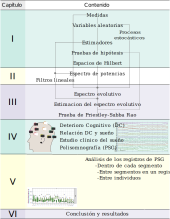
\includegraphics[width=.9\textwidth]{./estructura_texto_v2.pdf}
\caption[Estructura de la tesis]{Se ilustra gráficamente las \textit{dependencias} respecto a los tópicos de matemáticas, es decir, los temas que deben discutirse antes que otros. El resto del texto (incluyendo los tópicos de fisiología) son expuesto de forma más \textit{secuencial}, por lo que no se consideró necesario ilustrar sus dependencias.}
\label{intro:estructura}
\end{figure}

%%%%%%%%%%%%%%%%%%%%%%%%%%%%%%%%%%%%%%%%%%%%%%%%%%%%%%%%%%%%%%%%%%%%%%%%%%%%%%%%%%%%%%%%%%%%%%%%%%%
%%%%%%%%%%%%%%%%%%%%%%%%%%%%%%%%%%%%%%%%%%%%%%%%%%%%%%%%%%%%%%%%%%%%%%%%%%%%%%%%%%%%%%%%%%%%%%%%%%%